\section{Results}

\subsection{Results for longitudinal pump}

The longitudinal spatial wave function densities are depicted in Figure~\ref{long_eta} for different values of $\eta$.

\begin{figure}[htp]
\centering
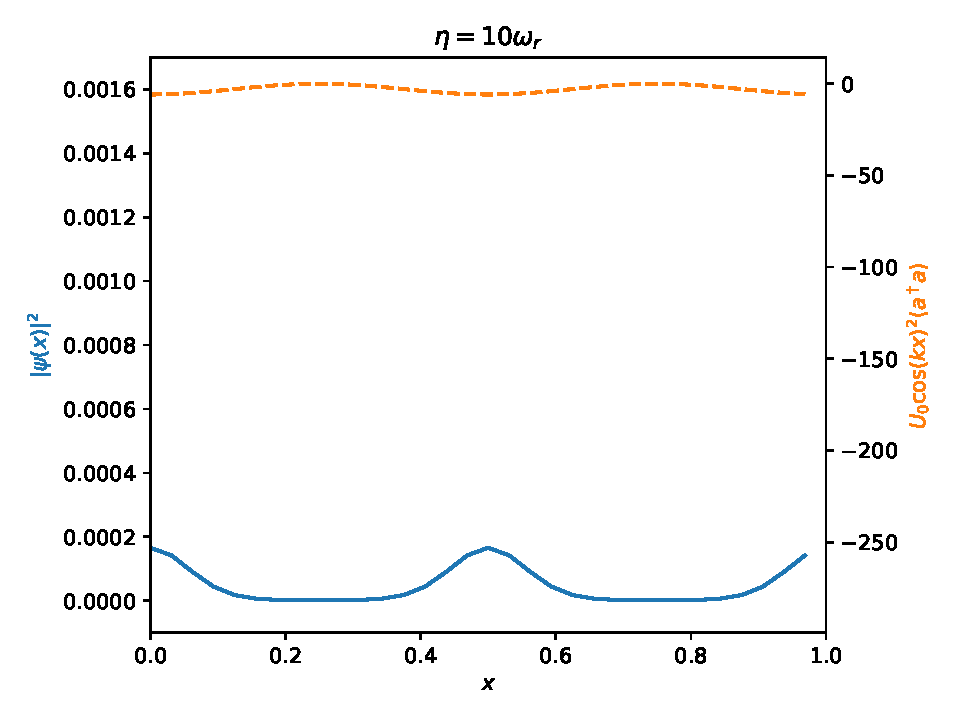
\includegraphics[width=.3\textwidth]{images/long_eta_10.pdf}\hfill
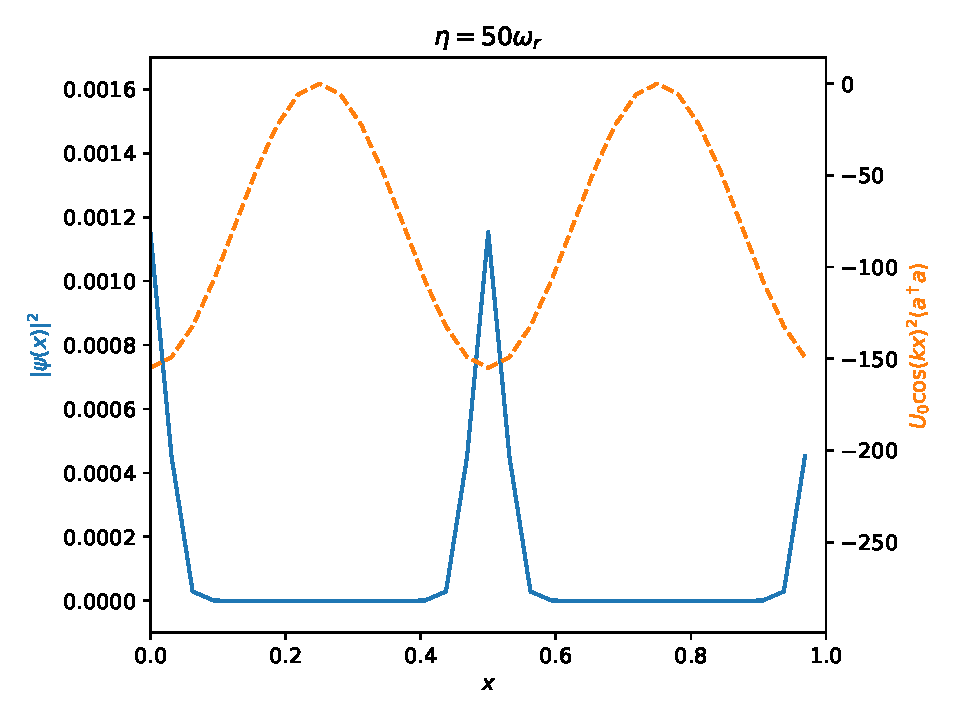
\includegraphics[width=.3\textwidth]{images/long_eta_50.pdf}\hfill
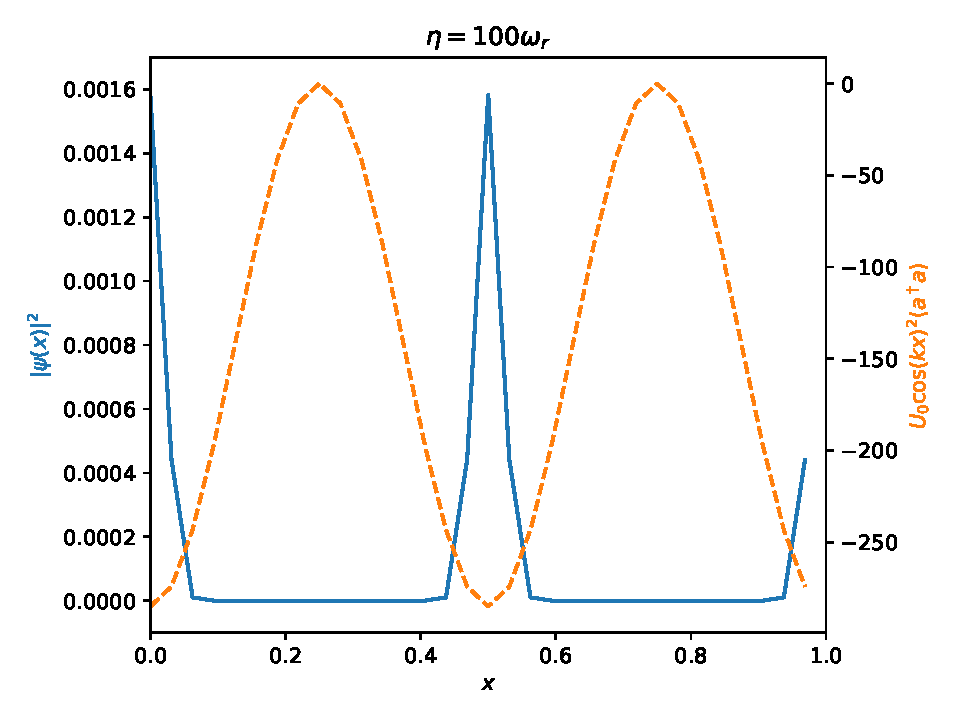
\includegraphics[width=.3\textwidth]{images/long_eta_100.pdf}
\caption{Longitudinal wave function densities for $\eta = 10 \omega_r$, $\eta = 50 \omega_r$ and $\eta = 100 \omega_r$.}
\label{long_eta}
\end{figure}
\FloatBarrier

\noindent Figures \ref{long_pmp_bunch} and \ref{trans_pmp_bunch} depict the bunching parameter $\langle \cos(kx)^2 \rangle$ each. We did not obtain any meaningful results with the order parameter $\langle \cos(kx) \rangle$.

\begin{figure}[ht]
  \centering
  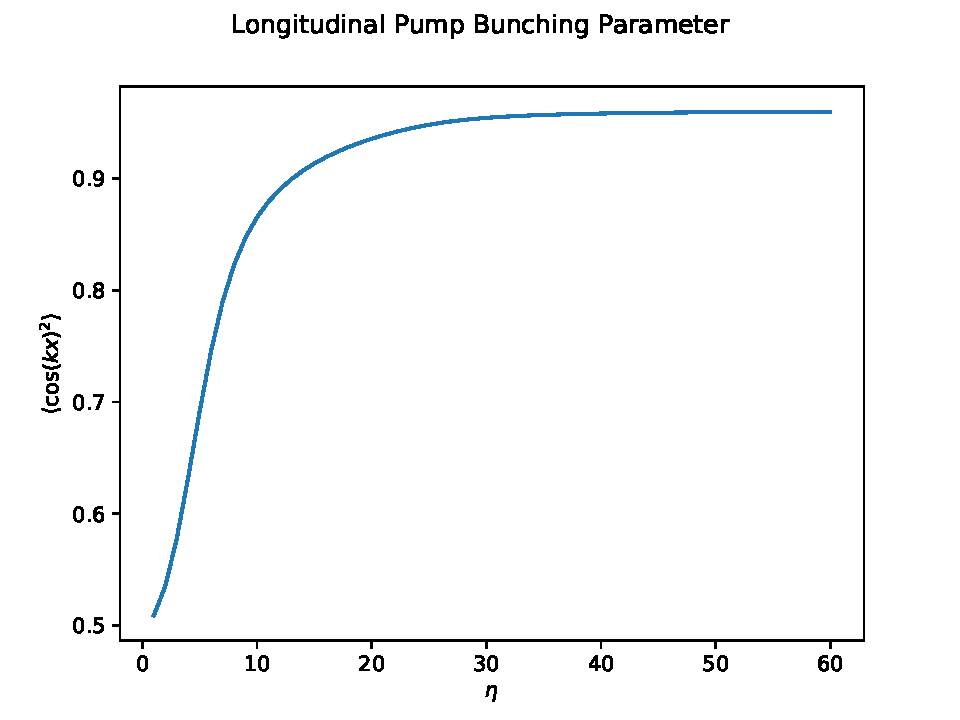
\includegraphics[width=.7\linewidth]{images/long_pmp_bunch.pdf}
  \caption{Bunching parameter for longitudinal pump with $\Delta_c = -10 \omega_r$ and $U_0 = -1 \omega_r$.}
  \label{long_pmp_bunch}
\end{figure}
\FloatBarrier

\noindent The momentum distribution can be seen in Figure~\ref{fig:long_momentum}.

\begin{figure}[ht]
  \centering
  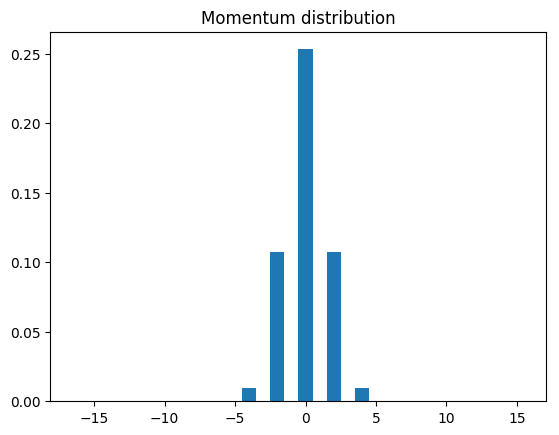
\includegraphics[width=.7\linewidth]{images/long_momentum.png}
  \caption{Momentum distribution for longitudinal pump.}
  \label{fig:long_momentum}
\end{figure}
\FloatBarrier

\noindent The photon number distribution can be seen in Figure~\ref{fig:long_photon_dist}.

\begin{figure}[ht]
  \centering
  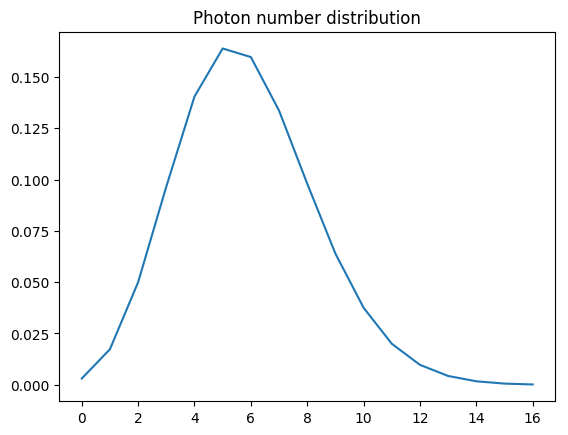
\includegraphics[width=.7\linewidth]{images/long_photon_dist.png}
  \caption{Photon number distribution for longitudinal pump.}
  \label{fig:long_photon_dist}
\end{figure}
\FloatBarrier

\subsection{Results for transversal pump}

\begin{figure}[ht]
  \centering
  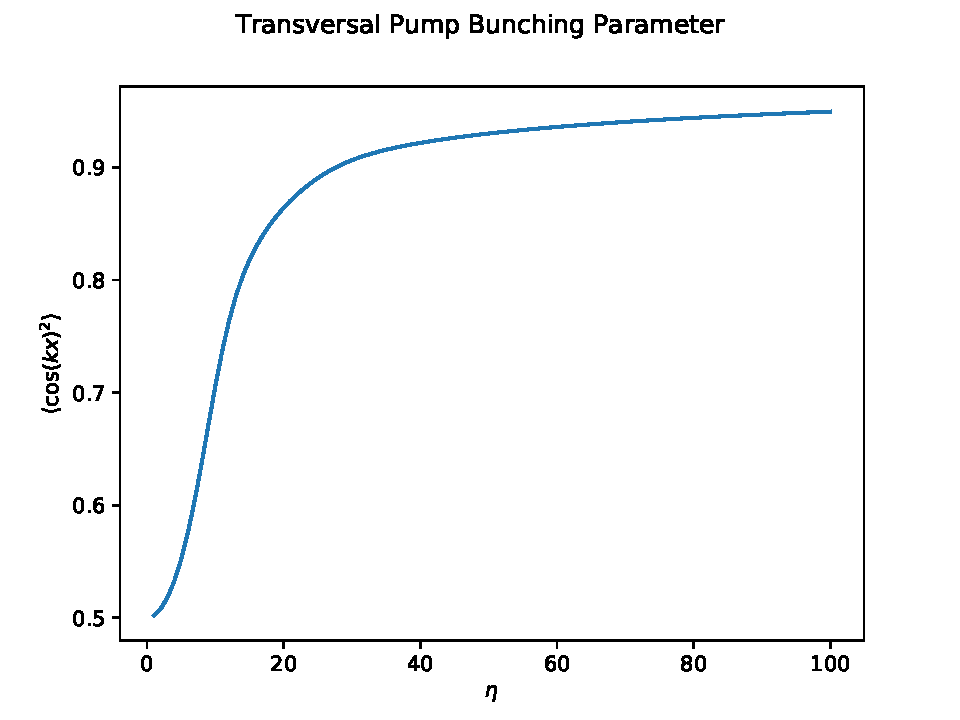
\includegraphics[width=.7\linewidth]{images/trans_pmp_bunch.pdf}
  \caption{Bunching parameter for transversal pump with $\Delta_c = -10 \omega_r$ and $U_0 = -1 \omega_r$.}
  \label{trans_pmp_bunch}
\end{figure}
\FloatBarrier

\noindent To obtain the order parameter as a function of $\eta$ for transversal pump, we used the mean-field approximation, as depicted in \cite{cold_atoms}. For now, a simple Euler algorithm will do. The results can be seen in Figure~\ref{trans_pmp_order}. Strangely, there is no threshold at which order sets in, but rather a gradual shift. We also tried to tweak the parameters similar to \cite{Nagy2008}, which unfortunately made the wave function all but disappear.

\begin{figure}[ht]
  \centering
  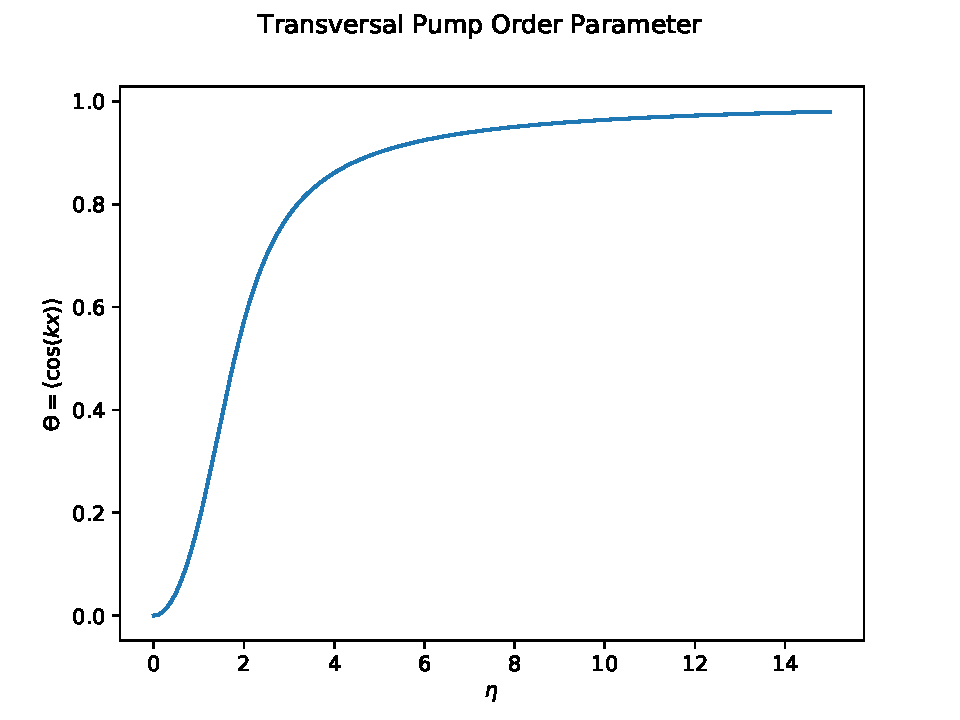
\includegraphics[width=.7\linewidth]{images/trans_pmp_order.pdf}
  \caption{Order parameter for transversal pump with $\Delta_c = -1 \omega_r$, $U_0 = -1 \omega_r$ and $\kappa = \omega_r$.}
  \label{trans_pmp_order}
\end{figure}
\FloatBarrier

\noindent The Husimi Q representation can be seen in Figure

\begin{figure}[ht]
  \centering
  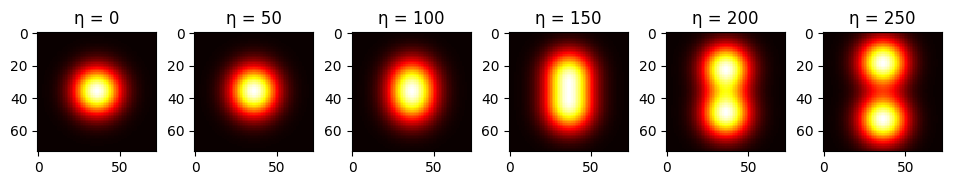
\includegraphics[width=.9\linewidth]{images/trans_qfunc.png}
  \caption{Husimi Q representation for the ground state at different pumping strengths.}
  \label{fig:trans_qfunc}
\end{figure}
\FloatBarrier